\documentclass[12pt]{article} % \documentclass{} is the first command in any LaTeX code.  It is used to define what kind of document you are creating such as an article or a book, and begins the document preamble

\usepackage{amsmath} % \usepackage is a command that allows you to add functionality to your LaTeX code

\usepackage[papersize={216mm,330mm},tmargin=20mm,bmargin=20mm,lmargin=20mm,rmargin=20mm]{geometry}
\usepackage[english]{babel}
\usepackage[utf8]{inputenc}
\usepackage{amsmath,amssymb,mathabx,amsthm}%\for eqref
\usepackage{lscape}
\usepackage{graphicx}
\usepackage{tikz}\usetikzlibrary{arrows.meta,calc} %library tikz
\usepackage{subcaption}


\usepackage{pgfplots}
\pgfplotsset{compat=1.15}
\usepackage{mathrsfs}
\usetikzlibrary{arrows}

\usepackage{color,soul} %package for highlining
\usepackage[colorinlistoftodos]{todonotes}
\usepackage{fancyhdr}
\usepackage{hyperref} %creat hyperlink
\hypersetup{
    colorlinks=true,
    linkcolor=blue,
    filecolor=magenta,      
    urlcolor=cyan,
    pdftitle={Overleaf Example},
    pdfpagemode=FullScreen,
    } %set up a hyperlink to be in blue 
\newtheorem{theorem}{Theorem}
\newtheorem{definition}{Definition}[section]
\newtheorem{prop}{Proposition}[section]
\newtheorem{lemma}{Lemma}[section]
\newtheorem*{remark}{Remark}

\pagestyle{fancy}
\cfoot{\thepage} % this is for the page numbering
\setlength\parindent{0pt} % noindent for the whole document.
\renewcommand{\baselinestretch}{1.1} % increase the distance between line.

\DeclareMathOperator{\SL2}{\text{SL}_2(\mathbb{R})}
\DeclareMathOperator{\sl2z}{SL_2(\mathbb{Z})}

\DeclareMathOperator{\SO}{SO_2(\mathbb{R})}
\DeclareMathOperator{\uH}{\mathfrak{H}}



\title{CHAPTER I : $\SL2$} % Sets article title
\date{\today} % Sets date for date compiled

% The preamble ends with the command \begin{document}
\begin{document} % All begin commands must be paired with an end command somewhere
\maketitle % creates a title using the information in the preamble (title, author, date)

In this chapter, I will give an exposition on the structure of $\SL2$ as the spaces of lattice, this space
plays the role of a toy model before exploring the space of lattice in the higher rank. The exposition follows
the paper \cite{} and  \cite{} closely.
\section{$\SL2$ and its action on the upper half plane $\uH$}
A priori, the upper half plane
\[\uH = \left\lbrace z: \Im z >0 \right\rbrace \subset \mathbb{C}\]
has no group structure on its. However, we will show below that it can identify topologically with the space
with the space of cosets $\SO\backslash\SL2$, and thus we can study the spaces $\uH$ via the spac of lattices $\SO\backslash\SL2$.
We define the action of $G= \SL2$ on $\uH$ as follows
\[
  \begin{bmatrix}a & b \\ c & d\end{bmatrix} \circ (z) = \frac{az + b}{cz + d}
\]
\begin{prop}
  The group $\SL2$ stabilizes \(\mathfrak{H}\) and acts transitively on it. In particular,
  \[
    \begin{bmatrix}1 & x \\ 0 & 1\end{bmatrix}\begin{bmatrix}\sqrt{y} & 0 \\ 0 & \frac{1}{\sqrt{y}}\end{bmatrix}(i) = x + iy \quad (\text{for } x \in \mathbb{R}, \, y > 0)
  \]
  Further, for \(g = \begin{bmatrix}a & b \\ c & d\end{bmatrix} \in SL_{2}(\mathbb{R})\) and \(z \in \mathfrak{H}\),
  \[
    \text{$\Im$}\,g(z) = \frac{\text{$\Im$}\,z}{|cz + d|^2}.
  \]
\end{prop}
\begin{proof}
  The first formula is clear. The second formula would imply that the upper half-plane is stabilized. Compute directly:
  \[
    2i \cdot \text{$\Im$} \left( \begin{pmatrix} a & b \\ c & d \end{pmatrix} (z) \right) = \frac{az + b}{cz + d} - \frac{d\overline{z} + b}{c\overline{z} + d} = \frac{(az + b)(c\overline{z} + d) - (a\overline{z} + b)(cz + d)}{|cz + d|^2}
  \]
  \[
    = \frac{adz - bc\overline{z} - bcz + ad\overline{z}}{|cz + d|^2} = \frac{z - \overline{z}}{|cz + d|^2}
  \]
  since \( ad - bc = 1 \).
\end{proof}
The point $z = i$ is special, in the sense that its stability group is the orthogonal group $K =\SO$. Indeed, for any \(g = \begin{bmatrix}a & b \\ c & d\end{bmatrix} \in SL_{2}(\mathbb{R})\)  we have
that
\[g \circ i = i \Leftrightarrow \dfrac{ai+b}{ci+d }=i \Leftrightarrow a=d \text{ and } b = -c \]
Combinining with the fact that $ad-bc=1$, we must have $a^2 + b^2=1$. This implies that there is a $\theta$ such that $a = \cos\theta$ and $b = \sin \theta$.
Since $G$ acts on $\uH$ transitively, we know from group theory that there is a bijection between the collection of cosets of
$\text{Stab}(i)$ in $G$ and the orbits of $i$. In particular
\begin{prop}
  We have an isomorphism of \(SL_{2}(\mathbb{R})\)-spaces
  \[
    \SO\backslash\SL2 \approx \mathfrak{H} \quad \text{via} \quad  SO(2)g \to g^{-1}(i)
  \]
  That is, the map respects the action of \(SL_{2}(\mathbb{R})\), in the sense that
  \[
    (\SO g)\cdot h \;\longrightarrow\; h^{-1}(g^{-1}i)
  \]
\end{prop}
\begin{proof}
  This is because of \textit{associativity}:
  \[
    (\SO g)\cdot h  = (\SO)\cdot (gh)  \;\longrightarrow\; (gh)^{-1}(i) = h^{-1}(g^{-1}(i))
  \]
  giving the result.
\end{proof}
\section{Fundamental domain for $\Gamma = SL_2(\mathbb{Z})$ on $\mathfrak{H}$}
Here is a picture of the fundamental domain $\mathfrak{H}/\Gamma$.
\[
  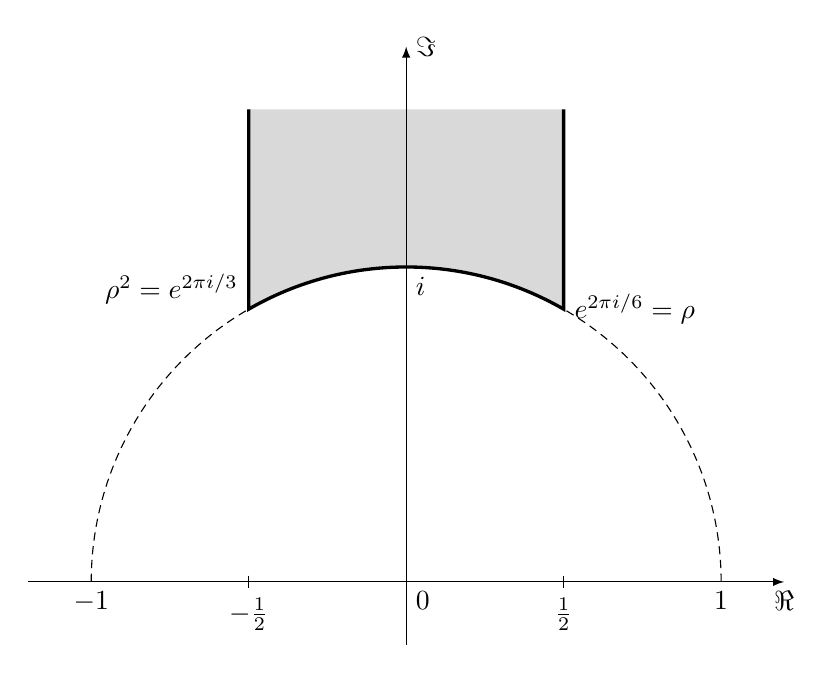
\begin{tikzpicture}[scale=4]
    \draw[densely dashed] (1,0) arc (0:60:1) (-1,0) arc (180:120:1);
    \draw[very thick, fill=gray!30] (.5,1.5) --node[right, pos=1]{$e^{2\pi i/6}=\rho$} (60:1) arc (60:120:1)
    --node[left, pos=.1]{$\rho^2=e^{2\pi i/3}$} (-.5,1.5);
    \draw[-latex] (-1.2,0) -- (1.2,0)node[below]{$\Re$};
    \draw[-latex] (0,-.2) -- (0,1.7)node[right]{$\Im$};
    \path(-1,0) --node[below, pos=0]{$-1$}node[below right, pos=.5]{0}node[below, pos=1]{1} (1,0)
    (0,1)node[below right]{$i$};
    \draw(-.5,.02)--(-.5,-.02)node[below]{$-\frac{1}{2}$}(.5,.02)--(.5,-.02)node[below]{$\frac{1}{2}$};
  \end{tikzpicture}\]
The goal of this section is to prove that under the action of the $\Gamma = \sl2z$, we can "move"
every points on the upper half plane to a domain, under an equivalence given by a specific action.
This is similar to the fundamental domain given by the translation action of $\mathbb{Z}$ to $\mathbb{R}$ is the half-open
unit interval $[0,1)$. In general, this give a simpler description to the homogenous space of lattice.

Note that when we try to compute the fundamental domain of $\mathbb{Z}\backslash \mathbb{R}$, we have $\mathbb{Z}$ plays a role of
\textit{discrete} subset of $\mathbb{R}$. We give a precise definition of discreteness as follows
\begin{definition}
  Let a group $G$ act continuously on a topological space $X$. A subset $\Gamma \subset G$ is called \textbf{discrete} if for any two compact subse
  $A,B$ in $X$, there are only finitely many $g \in \Gamma$ such that $g \circ A \cap B \ne \emptyset$.
\end{definition}
We will prove that the set
\[\Gamma = \sl2z = \left\lbrace \begin{bmatrix}
    a & b \\
    c & d
  \end{bmatrix} \in \SL2: a, b, c, d \in \mathbb{Z}\right\rbrace\]
is a discrete subgroup of $G = \SL2$.
To prove this, we first need the following lemma
\begin{lemma}\label{lm2}
  Fix a real number $r>0$ and $0<\delta<1$. We denote $R_{r,\delta}$ the rectangle
  \[R_{r,\delta} = \left\lbrace z = x+iy: -r \le x \le r, 0 <\delta \le y \le \delta^{-1}\right\rbrace\]
  Then for any $\epsilon >0$ and any fixed set $\mathbb{S}$ of coset representatives for $\Gamma_\infty\backslash \Gamma$, there are finitely
  many $g \in \mathbb{S}$ such that $\Im(g\circ z)>\epsilon$ for some $z \in R_{r,\delta}$.
\end{lemma}
In the above lemma, the notation $\Gamma_\infty$ is defined to be the set
\[ \Gamma_\infty = \left\lbrace\begin{bmatrix}
    1 & n \\
    0 & 1
  \end{bmatrix}: n \in \mathbb{Z} \right\rbrace.\] It can be seen easily that this is the
stability group of $\infty$ in $\mathfrak{H}$.
\begin{proof}
  Let \( g = \begin{bmatrix} a & b \\ c & d \end{bmatrix} \). Then for \( z \in R_{r, \delta} \),
  \[
    \text{Im}(g \circ z) = \frac{y}{c^2 y^2 + (cx + d)^2} < \epsilon
  \]
  if \( |c| > (y \epsilon)^{-\frac{1}{2}} \). On the other hand, for \( |c| \leq (y \epsilon)^{-\frac{1}{2}} \leq (\delta \epsilon)^{-\frac{1}{2}} \), we have
  \[
    \frac{y}{(cx + d)^2} < \epsilon
  \]
  if the following inequalities hold:
  \[
    |d| > |c| r + (y \epsilon^{-1})^{\frac{1}{2}} \geq |c| r + (\epsilon \delta)^{-\frac{1}{2}}.
  \]
  Consequently, \(\Im(g \circ z) > \epsilon\) only if
  \[
    |c| \leq (\delta \epsilon)^{-\frac{1}{2}} \quad \text{and} \quad |d| \leq (\epsilon \delta)^{-\frac{1}{2}} (r + 1),
  \]
  and the total number of such pairs (not counting $(c, d) = (0, \pm 1), (\pm 1, 0)$) is at most $\frac{4(r+1)} {(\epsilon \delta)}$. This proves the lemma.
\end{proof}
It follows from Lemma \ref{lm2} that $\Gamma = SL(2, \mathbb{Z})$ is a discrete subgroup of $SL(2, \mathbb{R})$. This is because:

\begin{enumerate}
  \item It is enough to show that for any compact subset $A \subset \mathfrak{H}$ there are only finitely many $g \in SL(2, \mathbb{Z})$ such that $(g \circ A) \cap A \neq \phi$;

  \item Every compact subset of $A \subset \mathfrak{H}$ is contained in a rectangle $R_{r,\delta}$ for some $r > 0$ and $0 < \delta < \delta^{-1}$;

  \item $((\alpha g) \circ R_{r,\delta}) \cap R_{r,\delta} = \phi$, except for finitely many $\alpha \in \Gamma_{\infty}$, $g \in \Gamma_{\infty}\backslash \Gamma$.
\end{enumerate}

To prove (3), note that Lemma \ref{lm2} implies that $(g \circ R_{r,\delta}) \cap R_{r,\delta} = \phi$ except for finitely many $g \in \Gamma_{\infty}\backslash \Gamma$. Let $S \subset \Gamma_{\infty}\backslash \Gamma$ denote this finite set of such elements $g$. If $g \not\in S$, then Lemma \ref{lm2} tells us that it is because $\Im(g \circ z) < \delta$ for all $z \in R_{r,\delta}$. Since $\Im(\alpha g \circ z) = \Im(g \circ z)$ for $\alpha \in \Gamma_{\infty}$, it is enough to show that for each $g \in S$, there are only finitely many $\alpha \in \Gamma_{\infty}$ such that $((\alpha g) \circ R_{r,\delta}) \cap R_{r,\delta} \neq \phi$. This last statement follows from the fact that $g \circ R_{r,\delta}$ itself lies in some other rectangle $R_{r',\delta'}$, and every $\alpha \in \Gamma_{\infty}$ is of the form $\alpha =
  \begin{bmatrix}
    1 & m \\
    0 & 1
  \end{bmatrix}
  (m \in \mathbb{Z})$, so that
\[
  \alpha \circ R_{r',\delta'} = \{x + iy \mid -r' + m \leq x \leq r' + m, \, 0 < \delta' \leq \delta''^{-1}\},
\]

which implies $(\alpha \circ R_{r',\delta'}) \cap R_{r,\delta} = \phi$ for $|m|$ sufficiently large.
Now we are ready to describe the fundamental domain for $\sl2z \backslash \uH$.
\begin{prop}\label{prop2}
  A fundamental domain for $\sl2z \backslash \uH$ can be given as the region
  \[\mathfrak{D} = \left\lbrace z=x+iy \in \uH: |z| \ge 1,-1/2 \le x \le 1/2 \right\rbrace \],
  modulo the congruent boundary points symmetric with respect to the imaginary axis.
\end{prop}
\begin{proof}
  First we eliminated the repeated points on the boundary. Note that the line $x = -1/2$ is the same as
  the line $x=1/2$ under the transformation $z \mapsto z+1$. Similarly, given a point on the circle
  $\left\lbrace |z|=1\right\rbrace$, the transformation $z \mapsto -|z|^{-1}$ satisfies
  \[\dfrac{-1}{x+iy} = \dfrac{-x+iy}{x^2+y^2}=-x+iy,\]
  which flips the sign of $x$. Thus it identifies the half circle on the right of the imaginary axis with that on the left.

  Now we need to show two things:
  \begin{enumerate}
    \item For any $z \in \uH$ we can find an element $g \in \sl2z$ such that $g\circ z \in \mathfrak{D}$.
    \item If $z \equiv z' \in \mathfrak{D}$ modulor $\sl2z$, then either $\Re(z)=\pm\frac{1}{2}$ and $z'=z\mp 1$, or
          $|z|=1$ and $z' = \frac{-1}{z} $.
  \end{enumerate}
  First we prove for (1): Fix $z \in \uH$. It follows from Lemma \ref{lm2} that for every $\epsilon > 0$, there are at most finitely many $g \in \mathrm{SL}(2, \mathbb{Z})$ such that $g \circ z$ lies in the strip
  \[
    D_{\epsilon} := \left\{ w \ \middle|\ -\frac{1}{2} \leq \mathrm{Re}(w) < \frac{1}{2},\ \epsilon \leq \mathrm{Im}(w) \right\}.
  \]
  Let $B_{\epsilon}$ denote the finite set of such $g \in \mathrm{SL}(2, \mathbb{Z})$.
  Clearly, for sufficiently small $\epsilon$, the set $B_{\epsilon}$ contains at least one element. We will show that there is at least one $g \in B_{\epsilon}$ such that $g \circ z \in D$. Among these finitely many $g \in B_{\epsilon}$, choose one such that $\Im(g \circ z)$ is maximal in $D_{\epsilon}$.
  If $|g \circ z| < 1$, then for $S = \begin{bmatrix} 0 & -1 \\ 1 & 0 \end{bmatrix}$, $T=\begin{bmatrix} 1 & 1 \\ 0 & 1 \end{bmatrix}$
  we have, for any $m$,
  \[\Im\left( T^mS g \circ z \right)= \Im\left(\dfrac{-1}{g\circ z}\right)=\dfrac{\Im(g\circ z)}{|g\circ z|^2} > \Im(g\circ z)\]
  But we can choose $m$ such that $T^m S g\circ z \in D_\epsilon$, which contradicts the maximality of $\Im(g\circ z)$.

  Next we give a proof for (2):Let $z \in D$, $g = \begin{bmatrix} a & b \\ c & d \end{bmatrix} \in \mathrm{SL}(2, \mathbb{Z})$, and assume that $g \circ z \in D$. Without loss of generality, we may assume that
  \[
    \Im(g \circ z) = \frac{y}{|cz + d|^2} \geq \Im(z),
  \]
  (otherwise just interchange $z$ and $g \circ z$ and use $g^{-1}$). This implies that $|cz + d| \leq 1$ which implies that $1 \geq |cy| \geq \frac{1}{\sqrt{3}}|c|$. This is clearly impossible if $|c| \geq 2$. So we only have to consider the cases $c = 0, \pm 1$. If $c = 0$ then $d = \pm 1$ and $g$ is a translation by $b$. Since $-\frac{1}{2} \leq \Re(z), \Re(g \circ z) \leq \frac{1}{2}$, this implies that either $b = 0$ and $z = g \circ z$ or else $b = \pm 1$ and $\Re(z) = \pm \frac{1}{2}$ while $\Re(g \circ z) = \mp \frac{1}{2}$. If $c = 1$, then $|z + d| \leq 1$ implies that $d = 0$ unless $z = e^{2\pi i / 3}$ and $d = 0, -1$. The case $d = 0$ implies that $|z| \leq 1$ which implies $|z| = 1$. Also, in this case, $c = 1$, $d = 0$, we must have $b = -1$ because $ad - bc = 1$. Then $g \circ z = a - \frac{1}{z + 1}$. It follows that $g \circ z = a - e^{2\pi i / 3}$ and $d = 1$, then we must have $a - b = 1$. It follows that $g \circ z = a - \frac{1}{z + 1} = a + e^{2\pi i / 3}$, which implies that $a = 0$ or 1. A similar argument holds when $z = e^{\pi i / 3}$ and $d = -1$. Finally, the case $c = -1$ can be reduced to the previous case $c = 1$ by reversing the signs of $a, b, c, d$.
\end{proof}
\section{Lattices and semi-stability in dimension $2$}
In this section, we investigate the notion of semi-stable lattices and how the
upper half plane $\uH$ can be regard as a spaces of two dimensional lattices.

Now regard $\mathbb{C} \cong \mathbb{R}^2$ via $x+iy \mapsto (x,y)$, and the inner product is defined to be
\[\left\langle z_1, z_2 \right\rangle = x_1x_2 + y_1y_2,\]
where $z_i= x_i+iy_i$. Now for any $z \in \uH$, the pair $(1,z)$ can be identified with the lattice
\[L_z = \mathbb{Z}z \oplus \mathbb{Z}\]
First we prove the following statement
\begin{prop}
  The upper half plane $\uH$ classifies similarity classes of two dimensional lattice.
\end{prop}
\begin{proof}
  Let $\mathbb{Z}e_1\oplus \mathbb{Z}e_2$ be any lattice in $\mathbb{R}_2$. Then using the
  above identification, we can find two complex number $z_1,z_2$ such that $|z_1| = ||e_1||$ and
  $|z_2| = \lvert e_2 \rvert$
  \todo{add this later, refer to the book by Anton Deitmar}
\end{proof}
Clearly in each classes of similar lattice, there is a unique one that has unit covolume.
The lattice spanned by $z$ and $1$ has volume $y$, so the corresponding unit lattice is the one spanned
by $z/\sqrt{y}$ and $1/\sqrt{y}$.

Using Proposition $\ref{prop2}$, it is immediate that every lattice spanned by $1$ and $z$
is similar to lattice generated by $1$ and a point $z'$ inside ther region $\mathfrak{D}$.

Historically, in two dimension, Proposition $\ref{prop2}$ is first discovered by Lagrange, with the distribution
of Gauss to solve for the shortest vector problem in two dimensional space. In the language of modern mathematics,
it can be phrased as follows:
\begin{prop}
  If $L$ is any lattice, and $u$ is a primitive vector in $L$, and $v'$ is a vector in the sublattice
  $L^\prime = L/\mathbb{Z}u$, then there exists a unique representative $v$ of $v'$ such that its projection onto $u$ lies in the interval
  $(-u/2,u/2]$. Moreover, the following inequality holds
  \[||v||^2 \le \dfrac{||u||^2}{4}+||v'||^2,\]
  where we identify $v'$ with a vector $v^\perp$ in the orthogonal complement of $u$.
\end{prop}
\begin{remark}
  Here the primitive vector is the vector such that it is not the multiple of any other vector in the lattice.
\end{remark}
An image to illustrate the above theorem \todo{Add figure}

To see why every point $z \in \uH$ can be transformed into a point inside $\mathfrak{D}$,
we start with a lattice generated by the $\mathbb{Z}$-linear combination of $1,z$ and
consider the shortest vector $u$. Applying the above lemma, we can find a vector $v$ with the length as least
as large as that of $u$. So if we rotate and scale to get $u=1$, the vector $v$ will lie
in the strip $(-1/2,1/2]$ and has the length at least 1. This clearly show that $v$ is a point in the domain
$\mathfrak{D}$.


\vspace{\baselineskip}
Now Grayson - following a prior idea of Stuhler - associated every lattice to a sort of \textbf{Newton Polygon}.
We will set up a graph coordinate in the following way:
\begin{enumerate}
  \item First we construct a two dimensional coordinate, say $Oxy$
  \item We highlight the origin.
  \item If we are dealing with the lattice $L$, compute the area of the fundamental domain of $L$
  \item Assign the point $(2, \log(vol(L)))$ to the line $x=2$ in the coordinate.
  \item If $v$ is any primitive vector, we put the point $(1,\log(v))$ in the set.
\end{enumerate}
Note that the lattice is discrete, so we can find a shortest vector $v$ of the lattice $L$. This will
correspond to the lowest point on the axis $x=1$ in the diagram. Note the that $x$-coordinate
of each of these point reflects its dimension.

As an example, let's consider the lattice of the following shape - with the shortest vector
$u$ has the length $||u||<1$.
\newpage
\begin{figure}[h]
  \centering
  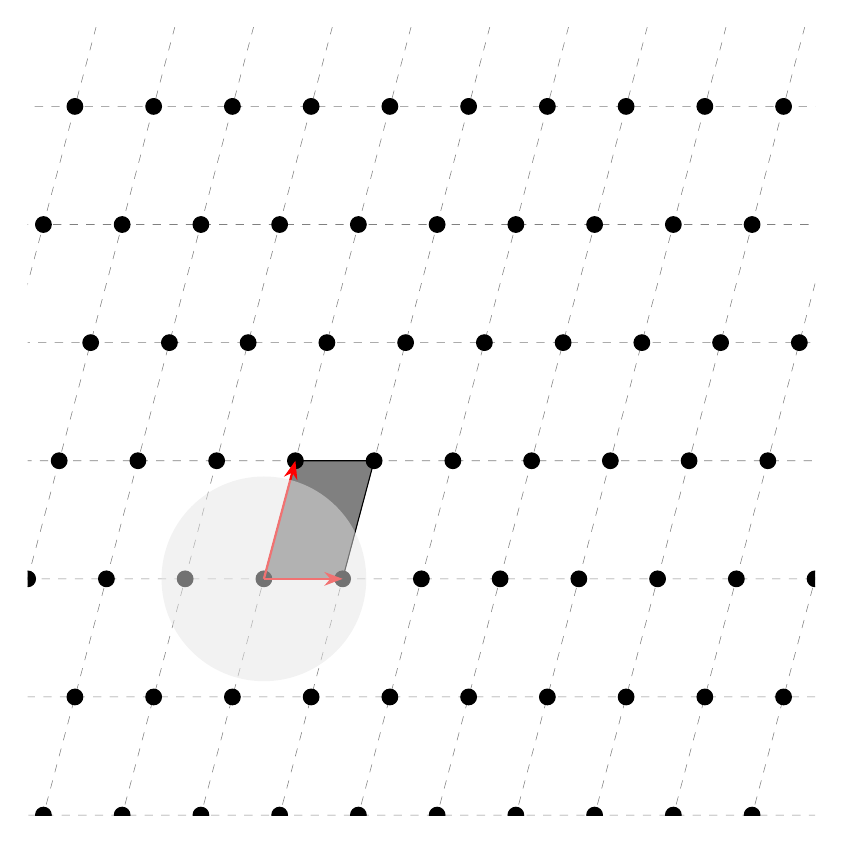
\begin{tikzpicture}
    \begin{scope}
      \clip (0,0) rectangle (10cm,10cm); % Clips the picture...
      \pgftransformcm{1}{0}{0.4}{1.5}{\pgfpoint{3cm}{3cm}} % Adjusted transformation matrix for less skew

      \draw[style=help lines,dashed] (-14,-14) grid[step=1cm] (14,14); % Draws a grid in the new coordinates
      \filldraw[fill=gray, draw=black] (0,0) rectangle (1,1); % Puts the shaded rectangle
      \foreach \x in {-7,-6,...,7}{                           % Two indices running over each
          \foreach \y in {-7,-6,...,7}{                       % node on the grid we have drawn 
              \node[draw,circle,inner sep=2pt,fill] at (\x,\y) {}; % Places a dot at those points
            }
        }
      % Draw the vector from (0,0) to (1,0) in the transformed coordinate system
      \draw[red, -Stealth, thick] (0,0) -- (1,0); % Vector from (0,0) to (1,0)
      \draw[red, -Stealth, thick] (0,0) -- (0,1); % Vector from (0,0) to (0,1)

    \end{scope}
    % Place the circle at the lowest-left vertex (3,3) in the original coordinate system
    \fill[gray!20,semitransparent] (3,3) circle (1.3cm); % Radius is 1.3cm to contain the shorter edge
  \end{tikzpicture}
  \caption{Example of a lattice}
  \label{fig:example}
\end{figure}
Now applying the above process, we get the figure on the left. If we further taking the convex hull of the diagram,
we will get the figure on the right
\begin{figure}[h]
  \centering
  \begin{minipage}{.2\textwidth}
    \begin{tikzpicture}[>=stealth, x=1.1cm, y=1.1cm]
      % Dashed lines (axes)
      \draw[help lines, dashed, ->] (-1,0) -- (3,0);
      \draw[help lines, dashed, ->] (0,-3) -- (0,3);
      \draw[help lines, dashed, ->] (1,-3) -- (1,3);
      \draw[help lines, dashed, ->] (2,-3) -- (2,3);

      % Points (all with fill=blue and radius=0.09cm)
      \filldraw[fill=blue] (2, -0.5) circle[radius=0.09cm];
      \filldraw[fill=blue] (0, 0) circle[radius=0.09cm]; % Removed duplicate
      \filldraw[fill=blue] (1, -0.7) circle[radius=0.09cm];

      \filldraw[fill=blue] (1, -0.3230737092181455) circle[radius=0.09cm];
      \filldraw[fill=blue] (1, 0.12122108098130914) circle[radius=0.09cm];
      \filldraw[fill=blue] (1, 2.28412917072110916) circle[radius=0.09cm];
      \filldraw[fill=blue] (1, 2.3729881287610001) circle[radius=0.09cm];
      \filldraw[fill=blue] (1, 0.4) circle[radius=0.09cm];
      \filldraw[fill=blue] (1, 0.5655158711807637) circle[radius=0.09cm];
      \filldraw[fill=blue] (1, 2.6445016116606668) circle[radius=0.09cm];
      \filldraw[fill=blue] (1, 0.7481703960405396) circle[radius=0.09cm];
      \filldraw[fill=blue] (1, 1.3282219276898275) circle[radius=0.09cm];
      \filldraw[fill=blue] (1, 1.0912647062501184) circle[radius=0.09cm];
      \filldraw[fill=blue] (1, 1.1603772291700336) circle[radius=0.09cm];
      \filldraw[fill=blue] (1, 1.2) circle[radius=0.09cm];
    \end{tikzpicture}~
  \end{minipage} \hspace{3cm} \begin{minipage}{.2\textwidth}
    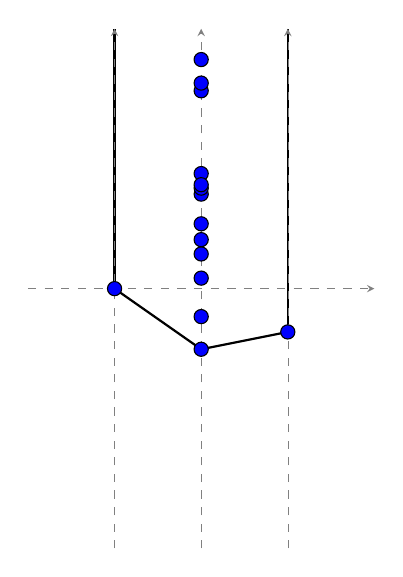
\begin{tikzpicture}[>=stealth, x=1.1cm, y=1.1cm]
      % Dashed lines (axes)
      \draw[help lines, dashed, ->] (-1,0) -- (3,0);
      \draw[thick] (0,0) -- (0,3);
      \draw[thick] (0,0) -- (1, -0.7);
      \draw[thick] (1,-0.7) -- (2,-0.5);
      \draw[thick]  (2,-0.5) -- (2,3);
      \draw[help lines, dashed, ->] (0,-3) -- (0,3);
      \draw[help lines, dashed, ->] (1,-3) -- (1,3);
      \draw[help lines, dashed, ->] (2,-3) -- (2,3);

      % Points (all with fill=blue and radius=0.09cm)
      \filldraw[fill=blue] (2, -0.5) circle[radius=0.09cm];
      \filldraw[fill=blue] (0, 0) circle[radius=0.09cm]; % Removed duplicate
      \filldraw[fill=blue] (1, -0.7) circle[radius=0.09cm];
      \filldraw[fill=blue] (1, -0.3230737092181455) circle[radius=0.09cm];
      \filldraw[fill=blue] (1, 0.12122108098130914) circle[radius=0.09cm];
      \filldraw[fill=blue] (1, 2.28412917072110916) circle[radius=0.09cm];
      \filldraw[fill=blue] (1, 2.3729881287610001) circle[radius=0.09cm];
      \filldraw[fill=blue] (1, 0.4) circle[radius=0.09cm];
      \filldraw[fill=blue] (1, 0.5655158711807637) circle[radius=0.09cm];
      \filldraw[fill=blue] (1, 2.6445016116606668) circle[radius=0.09cm];
      \filldraw[fill=blue] (1, 0.7481703960405396) circle[radius=0.09cm];
      \filldraw[fill=blue] (1, 1.3282219276898275) circle[radius=0.09cm];
      \filldraw[fill=blue] (1, 1.0912647062501184) circle[radius=0.09cm];
      \filldraw[fill=blue] (1, 1.1603772291700336) circle[radius=0.09cm];
      \filldraw[fill=blue] (1, 1.2) circle[radius=0.09cm];
    \end{tikzpicture}~
  \end{minipage}
\end{figure}
Clearly for each dimension, we have the corresponding lowest point, and so the convex hull of
the plot is bounded from below. Grayson calls the plot on the left \textbf{ canonical plot} of the lattice and
the boundary of the convex hull of the canonical plot its \textbf{canonical polygon}. In the expository \cite{}
of Bill Casselman, he instead calls the canonical polygon as \textbf{profile}. We will use the terminology of Casselman.

Now we will try to understand the profile of a lattice associated to a point $z \in \mathfrak{D}$. First we
prove a simple observation
\begin{lemma}
  If $z \in \mathfrak{D}$ then the lattice $L_z = \mathbb{Z}z\oplus \mathbb{Z}$ admits 1 as the shortest vector.
\end{lemma}
\begin{proof}
  We identify $z = x+iy$ with $(x,y) \in \mathbb{R}^2$ and $1$ with $(1,0) \in \mathbb{R}^2$.
  Assume that $1$ is not the shortest vector, then there exists $a,b \in \mathbb{Z}$ such that
  \[ |az+b|^2 < 1 \Leftrightarrow (ax+b)^2+(ay)^2 < 1\Leftrightarrow a^2|z|^2+2abx+b^2< 1\]
  Since $z \in \mathfrak{D}$, we clearly have $|x| \le \frac{1}{2}$ and $|z| \ge 1$,  thus the integers $a,b$ must
  satisfy
  \[ a^2 -|ab|+b^2 < 1\]
  Since the above expression are symmetric, we can assume $|a| \ge |b|$ and completing the square yields
  \[\left(\dfrac{\sqrt{3}b}{2}\right)^2 \ge a^2-ab+b^2 <1 \Rightarrow b^2<4/3 \Rightarrow b \le 1\]
  Subtituting $|b|=1$ yields $|a|^2-|a|<0$. There is no non-zero integer $a$ satifying this condition.
\end{proof}
Note that the area of the lattice $L_z$ is given by $\det\begin{bmatrix}
    y & x \\
    0 & 1
  \end{bmatrix} = y$. Note that we can scale the basis by a factor $a=\sqrt{y}$ so that we get a unique lattice.
So the lowest point with respect to the axis $x = 0,1,2$ are $(0,0), (1,-\log(a))$ and $(2,0)$.
The points of the interesting part of $\mathfrak{D}$ where $y\le 1$. This corresponds to the lattice
that has the canonical plot lying entirely on or above the $x-$axis. In particular, the profile of such lattice
only has the vertices at the origin and $(2,0)$. Grayson and Stuhler call these kind of lattice
\textbf{semi-stable}. If we don't normalize the area of such lattice then a semi-stable
lattice has the bottom of the profile as a straight line.
\vspace{\baselineskip}

Conversely, the lattice assigned to the points $z \in \uH$ with $\Im(z)>1$ correspond to the lattices
that has the canonical plot breaking at the lowest point on the axis $x=1$. In general case, this reflect the fact that
a non semi-stable lattice has the shortest vector $u$ satisfying $||u||<\sqrt{vol(L_z)}$. Follow Casselman,
we call such lattice \textbf{unstable}.
\end{document} % This is the end of the document
